\documentclass{standalone}
\usepackage{tikz}
\usetikzlibrary{patterns, positioning}


\begin{document}
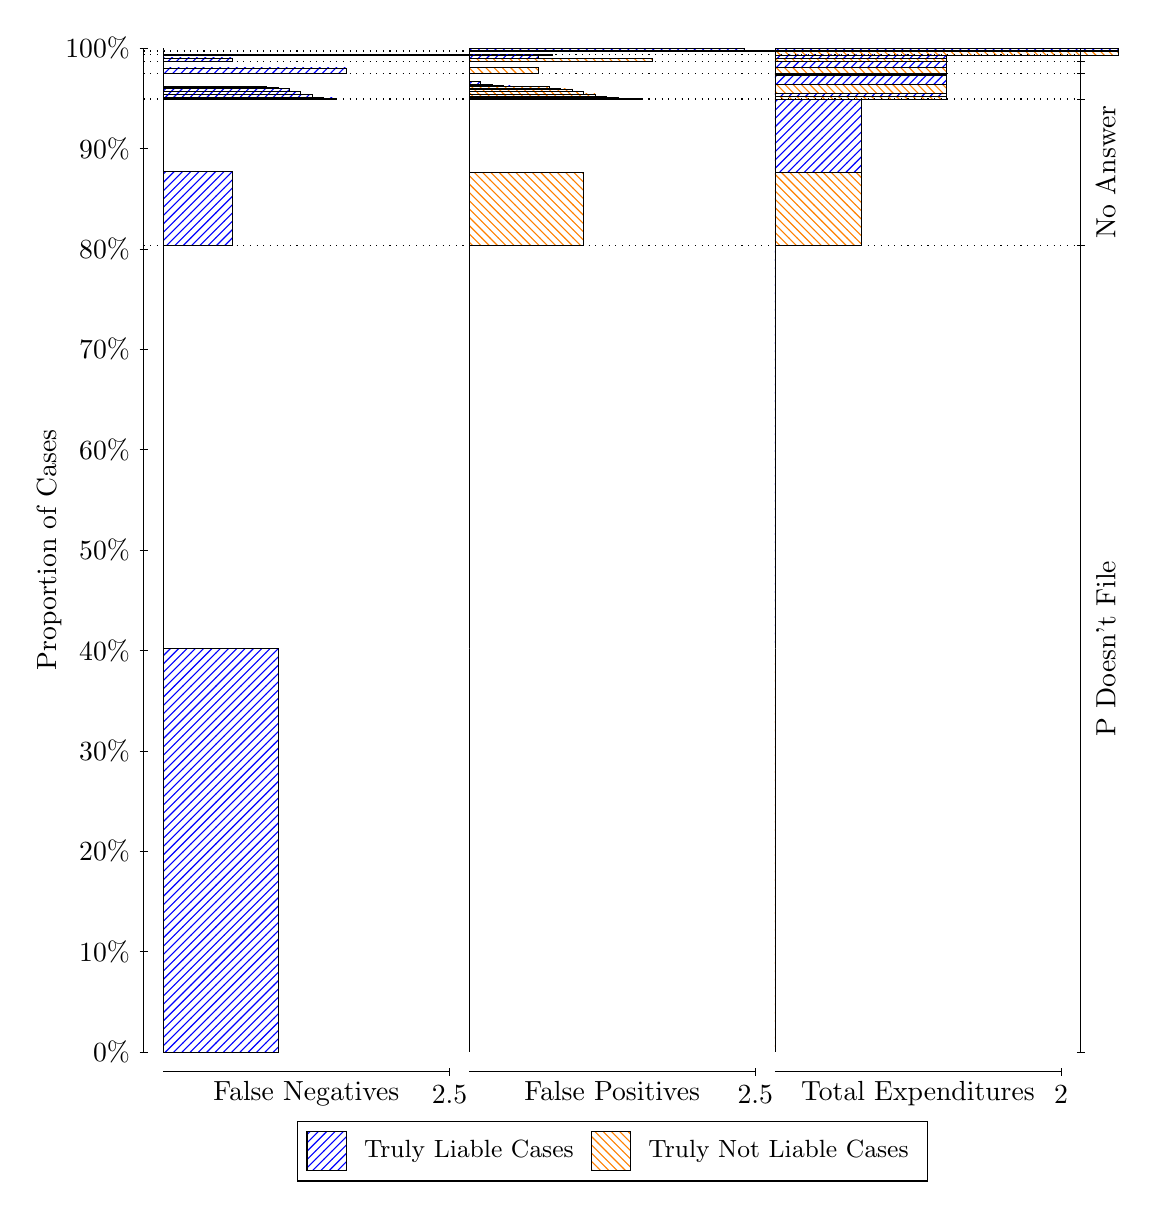
\begin{tikzpicture}
\draw[black, very thin] (1.5,1.75) -- (1.5,14.5);
\node[rotate=90, text=black, anchor=center] at (0.3, 8.125) {Proportion of Cases};
\draw[black, very thin] (1.45,1.75) -- (1.55,1.75);
\node[text=black, anchor=east] at (1.45, 1.75) {0\%};
\draw[black, very thin] (1.45,3.025) -- (1.55,3.025);
\node[text=black, anchor=east] at (1.45, 3.025) {10\%};
\draw[black, very thin] (1.45,4.3) -- (1.55,4.3);
\node[text=black, anchor=east] at (1.45, 4.3) {20\%};
\draw[black, very thin] (1.45,5.575) -- (1.55,5.575);
\node[text=black, anchor=east] at (1.45, 5.575) {30\%};
\draw[black, very thin] (1.45,6.85) -- (1.55,6.85);
\node[text=black, anchor=east] at (1.45, 6.85) {40\%};
\draw[black, very thin] (1.45,8.125) -- (1.55,8.125);
\node[text=black, anchor=east] at (1.45, 8.125) {50\%};
\draw[black, very thin] (1.45,9.4) -- (1.55,9.4);
\node[text=black, anchor=east] at (1.45, 9.4) {60\%};
\draw[black, very thin] (1.45,10.675) -- (1.55,10.675);
\node[text=black, anchor=east] at (1.45, 10.675) {70\%};
\draw[black, very thin] (1.45,11.95) -- (1.55,11.95);
\node[text=black, anchor=east] at (1.45, 11.95) {80\%};
\draw[black, very thin] (1.45,13.225) -- (1.55,13.225);
\node[text=black, anchor=east] at (1.45, 13.225) {90\%};
\draw[black, very thin] (1.45,14.5) -- (1.55,14.5);
\node[text=black, anchor=east] at (1.45, 14.5) {100\%};

\draw[black, very thin] (13.4,1.75) -- (13.4,14.5);
\draw[black, very thin] (13.35,1.75) -- (13.45,1.75);
\node[anchor=west] at (13.35, 1.75) {};
\draw[black, very thin] (13.35,11.995) -- (13.45,11.995);
\node[anchor=west] at (13.35, 11.995) {};
\draw[black, very thin] (13.35,13.852) -- (13.45,13.852);
\node[anchor=west] at (13.35, 13.852) {};
\draw[black, very thin] (13.35,14.176) -- (13.45,14.176);
\node[anchor=west] at (13.35, 14.176) {};
\draw[black, very thin] (13.35,14.33) -- (13.45,14.33);
\node[anchor=west] at (13.35, 14.33) {};
\draw[black, very thin] (13.35,14.414) -- (13.45,14.414);
\node[anchor=west] at (13.35, 14.414) {};
\draw[black, very thin] (13.35,14.462) -- (13.45,14.462);
\node[anchor=west] at (13.35, 14.462) {};
\draw[black, very thin] (13.35,14.5) -- (13.45,14.5);
\node[anchor=west] at (13.35, 14.5) {};

\draw[black, very thin, pattern color=blue, pattern=north east lines] (1.75,1.75) rectangle (3.2033,6.8723);
\draw[black, very thin, pattern color=orange, pattern=north west lines] (1.75,6.8723) rectangle (1.75,11.995);
\draw[black, very thin, pattern color=blue, pattern=north east lines] (1.75,11.995) rectangle (2.622,12.929);
\draw[black, very thin, pattern color=orange, pattern=north west lines] (1.75,12.929) rectangle (1.75,13.852);
\draw[black, very thin, pattern color=blue, pattern=north east lines] (1.75,13.852) rectangle (3.93,13.868);
\draw[black, very thin, pattern color=blue, pattern=north east lines] (1.75,13.868) rectangle (3.7847,13.876);
\draw[black, very thin, pattern color=blue, pattern=north east lines] (1.75,13.876) rectangle (3.6393,13.911);
\draw[black, very thin, pattern color=blue, pattern=north east lines] (1.75,13.911) rectangle (3.494,13.95);
\draw[black, very thin, pattern color=blue, pattern=north east lines] (1.75,13.95) rectangle (3.3487,13.987);
\draw[black, very thin, pattern color=blue, pattern=north east lines] (1.75,13.987) rectangle (3.2033,13.999);
\draw[black, very thin, pattern color=blue, pattern=north east lines] (1.75,13.999) rectangle (3.058,14.008);
\draw[black, very thin, pattern color=blue, pattern=north east lines] (1.75,14.008) rectangle (2.9127,14.012);
\draw[black, very thin, pattern color=blue, pattern=north east lines] (1.75,14.012) rectangle (2.7673,14.017);
\draw[black, very thin, pattern color=orange, pattern=north west lines] (1.75,14.017) rectangle (1.75,14.176);
\draw[black, very thin, pattern color=blue, pattern=north east lines] (1.75,14.176) rectangle (4.0753,14.247);
\draw[black, very thin, pattern color=orange, pattern=north west lines] (1.75,14.247) rectangle (1.75,14.33);
\draw[black, very thin, pattern color=blue, pattern=north east lines] (1.75,14.33) rectangle (2.622,14.374);
\draw[black, very thin, pattern color=orange, pattern=north west lines] (1.75,14.374) rectangle (1.75,14.414);
\draw[black, very thin, pattern color=blue, pattern=north east lines] (1.75,14.414) rectangle (6.6913,14.422);
\draw[black, very thin, pattern color=orange, pattern=north west lines] (1.75,14.422) rectangle (1.75,14.462);
\draw[black, very thin, pattern color=orange, pattern=north west lines] (1.75,14.462) rectangle (1.75,14.47);
\draw[black, very thin, pattern color=blue, pattern=north east lines] (1.75,14.47) rectangle (1.75,14.5);
\draw[black, very thin, pattern color=orange, pattern=north west lines] (5.6333,1.75) rectangle (5.6333,6.8725);
\draw[black, very thin, pattern color=blue, pattern=north east lines] (5.6333,6.8725) rectangle (5.6333,11.995);
\draw[black, very thin, pattern color=orange, pattern=north west lines] (5.6333,11.995) rectangle (7.0867,12.918);
\draw[black, very thin, pattern color=blue, pattern=north east lines] (5.6333,12.918) rectangle (5.6333,13.852);
\draw[black, very thin, pattern color=orange, pattern=north west lines] (5.6333,13.852) rectangle (7.8133,13.856);
\draw[black, very thin, pattern color=orange, pattern=north west lines] (5.6333,13.856) rectangle (7.668,13.86);
\draw[black, very thin, pattern color=orange, pattern=north west lines] (5.6333,13.86) rectangle (7.5227,13.87);
\draw[black, very thin, pattern color=orange, pattern=north west lines] (5.6333,13.87) rectangle (7.3773,13.882);
\draw[black, very thin, pattern color=orange, pattern=north west lines] (5.6333,13.882) rectangle (7.232,13.917);
\draw[black, very thin, pattern color=orange, pattern=north west lines] (5.6333,13.917) rectangle (7.0867,13.951);
\draw[black, very thin, pattern color=orange, pattern=north west lines] (5.6333,13.951) rectangle (6.9413,13.982);
\draw[black, very thin, pattern color=orange, pattern=north west lines] (5.6333,13.982) rectangle (6.796,13.99);
\draw[black, very thin, pattern color=orange, pattern=north west lines] (5.6333,13.99) rectangle (6.6507,14.011);
\draw[black, very thin, pattern color=blue, pattern=north east lines] (5.6333,14.011) rectangle (6.36,14.015);
\draw[black, very thin, pattern color=blue, pattern=north east lines] (5.6333,14.015) rectangle (6.2147,14.02);
\draw[black, very thin, pattern color=blue, pattern=north east lines] (5.6333,14.02) rectangle (6.0693,14.029);
\draw[black, very thin, pattern color=blue, pattern=north east lines] (5.6333,14.029) rectangle (5.924,14.041);
\draw[black, very thin, pattern color=blue, pattern=north east lines] (5.6333,14.041) rectangle (5.7787,14.078);
\draw[black, very thin, pattern color=blue, pattern=north east lines] (5.6333,14.078) rectangle (5.6333,14.176);
\draw[black, very thin, pattern color=orange, pattern=north west lines] (5.6333,14.176) rectangle (6.5053,14.259);
\draw[black, very thin, pattern color=blue, pattern=north east lines] (5.6333,14.259) rectangle (5.6333,14.33);
\draw[black, very thin, pattern color=orange, pattern=north west lines] (5.6333,14.33) rectangle (7.9587,14.369);
\draw[black, very thin, pattern color=blue, pattern=north east lines] (5.6333,14.369) rectangle (6.5053,14.414);
\draw[black, very thin, pattern color=orange, pattern=north west lines] (5.6333,14.414) rectangle (5.6333,14.453);
\draw[black, very thin, pattern color=blue, pattern=north east lines] (5.6333,14.453) rectangle (5.6333,14.462);
\draw[black, very thin, pattern color=orange, pattern=north west lines] (5.6333,14.462) rectangle (10.575,14.47);
\draw[black, very thin, pattern color=blue, pattern=north east lines] (5.6333,14.47) rectangle (9.1213,14.5);
\draw[black, very thin, pattern color=orange, pattern=north west lines] (9.5167,1.75) rectangle (9.5167,6.8725);
\draw[black, very thin, pattern color=blue, pattern=north east lines] (9.5167,6.8725) rectangle (9.5167,11.995);
\draw[black, very thin, pattern color=orange, pattern=north west lines] (9.5167,11.995) rectangle (10.607,12.918);
\draw[black, very thin, pattern color=blue, pattern=north east lines] (9.5167,12.918) rectangle (10.607,13.852);
\draw[black, very thin, pattern color=orange, pattern=north west lines] (9.5167,13.852) rectangle (11.697,13.887);
\draw[black, very thin, pattern color=blue, pattern=north east lines] (9.5167,13.887) rectangle (11.697,13.924);
\draw[black, very thin, pattern color=orange, pattern=north west lines] (9.5167,13.924) rectangle (11.697,14.034);
\draw[black, very thin, pattern color=blue, pattern=north east lines] (9.5167,14.034) rectangle (11.697,14.148);
\draw[black, very thin, pattern color=orange, pattern=north west lines] (9.5167,14.148) rectangle (11.697,14.162);
\draw[black, very thin, pattern color=blue, pattern=north east lines] (9.5167,14.162) rectangle (11.697,14.176);
\draw[black, very thin, pattern color=orange, pattern=north west lines] (9.5167,14.176) rectangle (11.697,14.259);
\draw[black, very thin, pattern color=blue, pattern=north east lines] (9.5167,14.259) rectangle (11.697,14.33);
\draw[black, very thin, pattern color=orange, pattern=north west lines] (9.5167,14.33) rectangle (11.697,14.369);
\draw[black, very thin, pattern color=blue, pattern=north east lines] (9.5167,14.369) rectangle (11.697,14.414);
\draw[black, very thin, pattern color=orange, pattern=north west lines] (9.5167,14.414) rectangle (13.877,14.453);
\draw[black, very thin, pattern color=blue, pattern=north east lines] (9.5167,14.453) rectangle (13.877,14.462);
\draw[black, very thin, pattern color=orange, pattern=north west lines] (9.5167,14.462) rectangle (13.877,14.47);
\draw[black, very thin, pattern color=blue, pattern=north east lines] (9.5167,14.47) rectangle (13.877,14.5);
\draw[black, dotted] (1.5,11.995) -- (13.4,11.995);
\draw[black, dotted] (1.5,13.852) -- (13.4,13.852);
\draw[black, dotted] (1.5,14.176) -- (13.4,14.176);
\draw[black, dotted] (1.5,14.33) -- (13.4,14.33);
\draw[black, dotted] (1.5,14.414) -- (13.4,14.414);
\draw[black, dotted] (1.5,14.462) -- (13.4,14.462);
\draw[black, very thin] (1.75,1.5) -- (5.3833,1.5);
\node[text=black, anchor=north] at (3.5667, 1.5) {False Negatives};
\draw[black, very thin] (5.3833,1.45) -- (5.3833,1.55);
\node[text=black, anchor=north] at (5.3833, 1.45) {2.5};

\draw[black, very thin] (5.6333,1.5) -- (9.2667,1.5);
\node[text=black, anchor=north] at (7.45, 1.5) {False Positives};
\draw[black, very thin] (9.2667,1.45) -- (9.2667,1.55);
\node[text=black, anchor=north] at (9.2667, 1.45) {2.5};

\draw[black, very thin] (9.5167,1.5) -- (13.15,1.5);
\node[text=black, anchor=north] at (11.333, 1.5) {Total Expenditures};
\draw[black, very thin] (13.15,1.45) -- (13.15,1.55);
\node[text=black, anchor=north] at (13.15, 1.45) {2};

\node[text=black, centered, rotate=90] at (13.72, 6.8724) {P Doesn't File};
\node[text=black, centered, rotate=90] at (13.72, 12.923) {No Answer};






\draw (7.449999999999999,1.5) node[draw=none] (baseCoordinate) {};
\begin{scope}[align=center]
        \matrix[scale=0.5, draw=black, below=0.5cm of baseCoordinate, nodes={draw}, column sep=0.1cm]{
            \node[rectangle, draw, minimum width=0.5cm, minimum height=0.5cm, pattern color=blue, pattern=north east lines] {}; &
            \node[draw=none, font=\small, text=black] (B) {Truly Liable Cases}; &
            \node[rectangle, draw, minimum width=0.5cm, minimum height=0.5cm, pattern color=orange, pattern=north west lines] {}; &
            \node[draw=none, font=\small, text=black] (B) {Truly Not Liable Cases}; \\
            };
\end{scope}

\end{tikzpicture}
\end{document}